\section{Front-end}
\label{sec:front-end}
\subsection{Initial Ideas}

The main idea for the user interface is to keep it simple and user-friendly without loosing advanced functionality. Initially we started making a rough drawing - so to better understand what we were dealing with (See figure \ref{fig:initial_idea_frontend}). Doing so we tried to plan ahead on how the visuals could look like, the functionality, and how users would be able to control the policy engine.

\begin{figure}[h!]
\centering
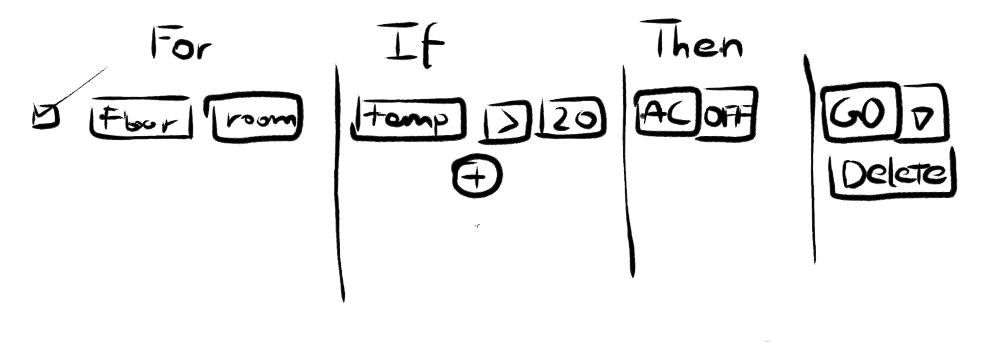
\includegraphics[width=\columnwidth]{initial_idea_frontend.png}
\caption{Drawing the initial idea of the element needed on the website, so a user can create, delete or modify a policy.}
\label{fig:initial_idea_frontend}
\end{figure}

We quickly realized that our ideas could easily expand the project, with numerous functionality and features, that would bring the project to a far more complex level.
We mapped all our ideas and prioritised them, and made a selection of ideas, which we planned on implementing.

The selected ideas included that:
\begin{itemize}
\item Users should be able to add, delete and modify policies.
\item Users should be able to use complex operators in policies.
\item Users should be able to create nested rules in policies.
\item Users should be able to use wildcards in a policy (effecting for instance an entire floor without the need to specify the rooms that belong to the chosen floor).
\item Users should be able to save policies and easily toggle an ON or OFF state.
\item Users should be able to combine multiple sensors in a single policy.
\end{itemize}


The ideas were broken into three main front-end sites\footnote{Front-end "sites" are dynamic HTML website.}, from where the user can control the policy engine and overlook its operation.

The three mains are:
\begin{enumerate}
\item A site where a user can create, delete or modify -policies.
\item A site that visually represent the building digitally with floors and rooms (like a map used to navigate through rooms and floors).
\item A site that displays sensor values and group them in regards to the individual room they represent.
\end{enumerate}
	

\subsection{Usability}
Seeing policies as rules for rooms in a building, with multiple sensors in each and every room, that can affect multiple actuators - not only in one room, but all of the rooms in a building: It leaves the user with a lot of selections. 
This will, if not represented properly, complex the process of adding new policies.

Following the principles of Steve Krug's "Don't Make Me Think: Common Sense Approach to the Web"\cite{Krug:2005:DMM:1051204}, the functionality of a website should always let users accomplish their intended tasks as easy and directly as possible.
Throughout the development of the front-end sites we have thrived to do so.

As an example, we have designed the process of adding new policies, as stepwise selections, instead of presenting the users with all the capabilities and elements at once.
The task then looks simpler, and makes the flow of  adding a new policy, more easy, and more direct.

\begin{figure}[h!]
\centering
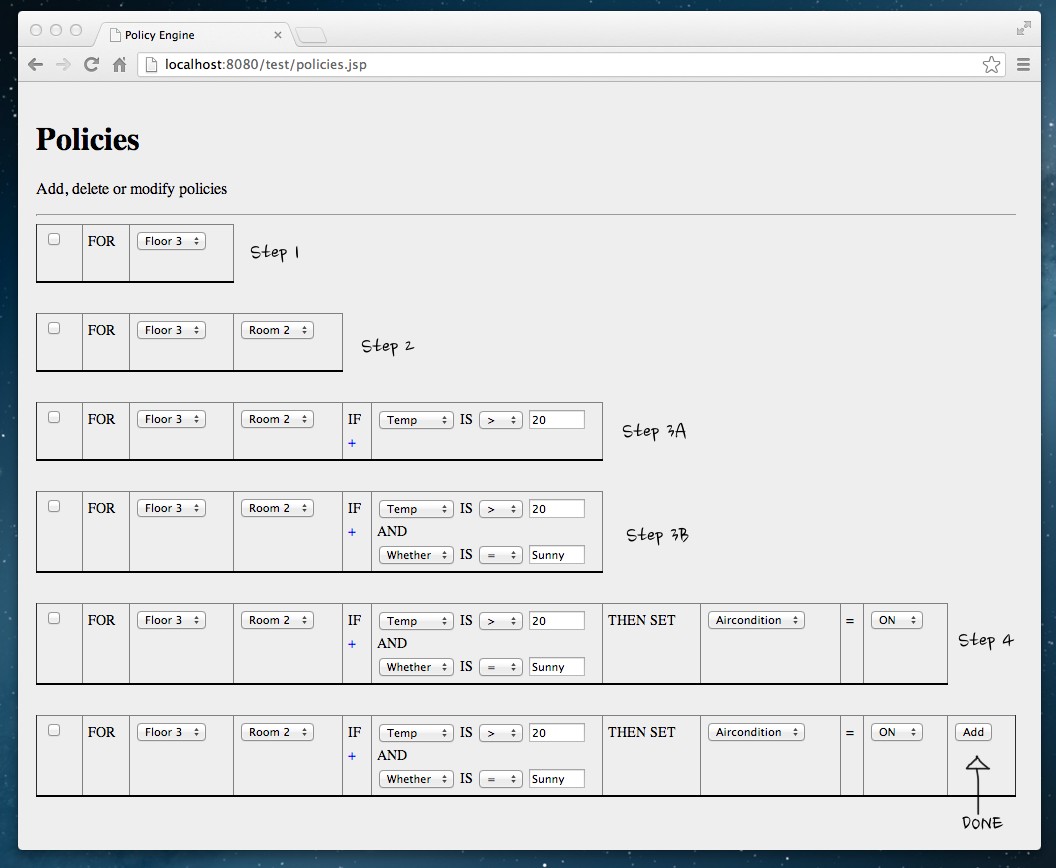
\includegraphics[width=\columnwidth]{building_policy_steps.png}
\caption{Illustrating the different elements introduced step-by-step. When the user has selected the first elements in "Step 1", then the elements in "Step 2" appears, and so it continues until a final "Add" button completes the process.}
\label{fig:building_policy_steps}
\end{figure}

Another approach towards usability was using web elements like: Selectors and Buttons, instead of having textual policies, and thereby forcing users to write policy, using the keyboard.

For a developer textual editing and console commands might be preferred, and may somewhat be quicker, while they know the inputs by heart. But the intended users of our policy engine, are most likely not developers or fans of typing in commands.
Also it forces users to memorize the inputs, and makes controlling the policy engine less intuitive. Therefore the idea was discarded and visual elements was implemented instead.

As for a future version of the policy engine, both methods could be implemented to function in parallel, giving a user both choices, and also the capability of copy and paste policies quickly.